\subsection{Shell}

\begin{center}
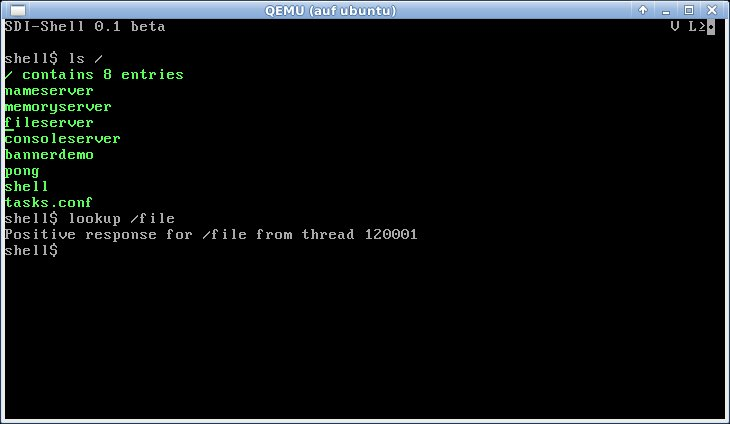
\includegraphics[scale=0.65]{shell}
\end{center}

Beim Systemstart wird auf den Konsolen 2 bis 8 jeweils eine Shell gestartet. Die Shell verfügt über folgende Builtins:

\begin{itemize}
	\item ls: Auflisten eines Directories auf dem Fileserver
	\item cat: Auslesen einer Datei vom Fileserver und Ausgabe auf der Konsole
	\item lookup: Auflösen von Pfaden über das Naming
	\item uname: Ausgabe der Systemversion
\end{itemize}

Wird ein Kommando aufgerufen, welches nicht als builtin bekannt ist, versucht die Shell, dieses über den Taskserver zu starten.
